\subsection{Genotype Size and Genotype Mutations}

Figure~\ref{fig:Size} shows the evolution of genotype size under the 4 types of environmental fluctuations. The imposed size limit of 50 program statements tends to blur the differences between the different scenarios since most simulations converge to this limit. Yet, ScF clearly restricts the size of the genotypes more severely than SE, LF and SF, while these other conditions do not appear to influence genotype size. This size reduction by ScF could be a way to increase the impact of genotypic mutations on the phenotype. This is because, even though the number of statements potentially affected by mutations in LGP increases proportionally with genotype size, hence could have a larger effect on the phenotype, there can also be a ``buffer'' effect brought by information redundancy in longer genotypes, which would in fact stabilize the phenotype. Hence, mutations in more compact genomes might end up being more impactful\footnote{Extra analysis of the effective length, very similar regardless of the setting, backup this idea.}.

Figure~\ref{fig:Mutations} depicts the amount of mutations separating the current MCG from individuals created during initialization. It is not surprising that more mutations are selected for when environmental fluctuations are introduced, and their number seem to depend more on the strength of these fluctuations (i.e. the contrast between two successive propagation probability patterns $E$) rather than their periodicity. We also note that the proximity of SF and ScF indicates that their differences in size are not explained by differences in the number of selected mutations.

\begin{figure}[h]
\centering
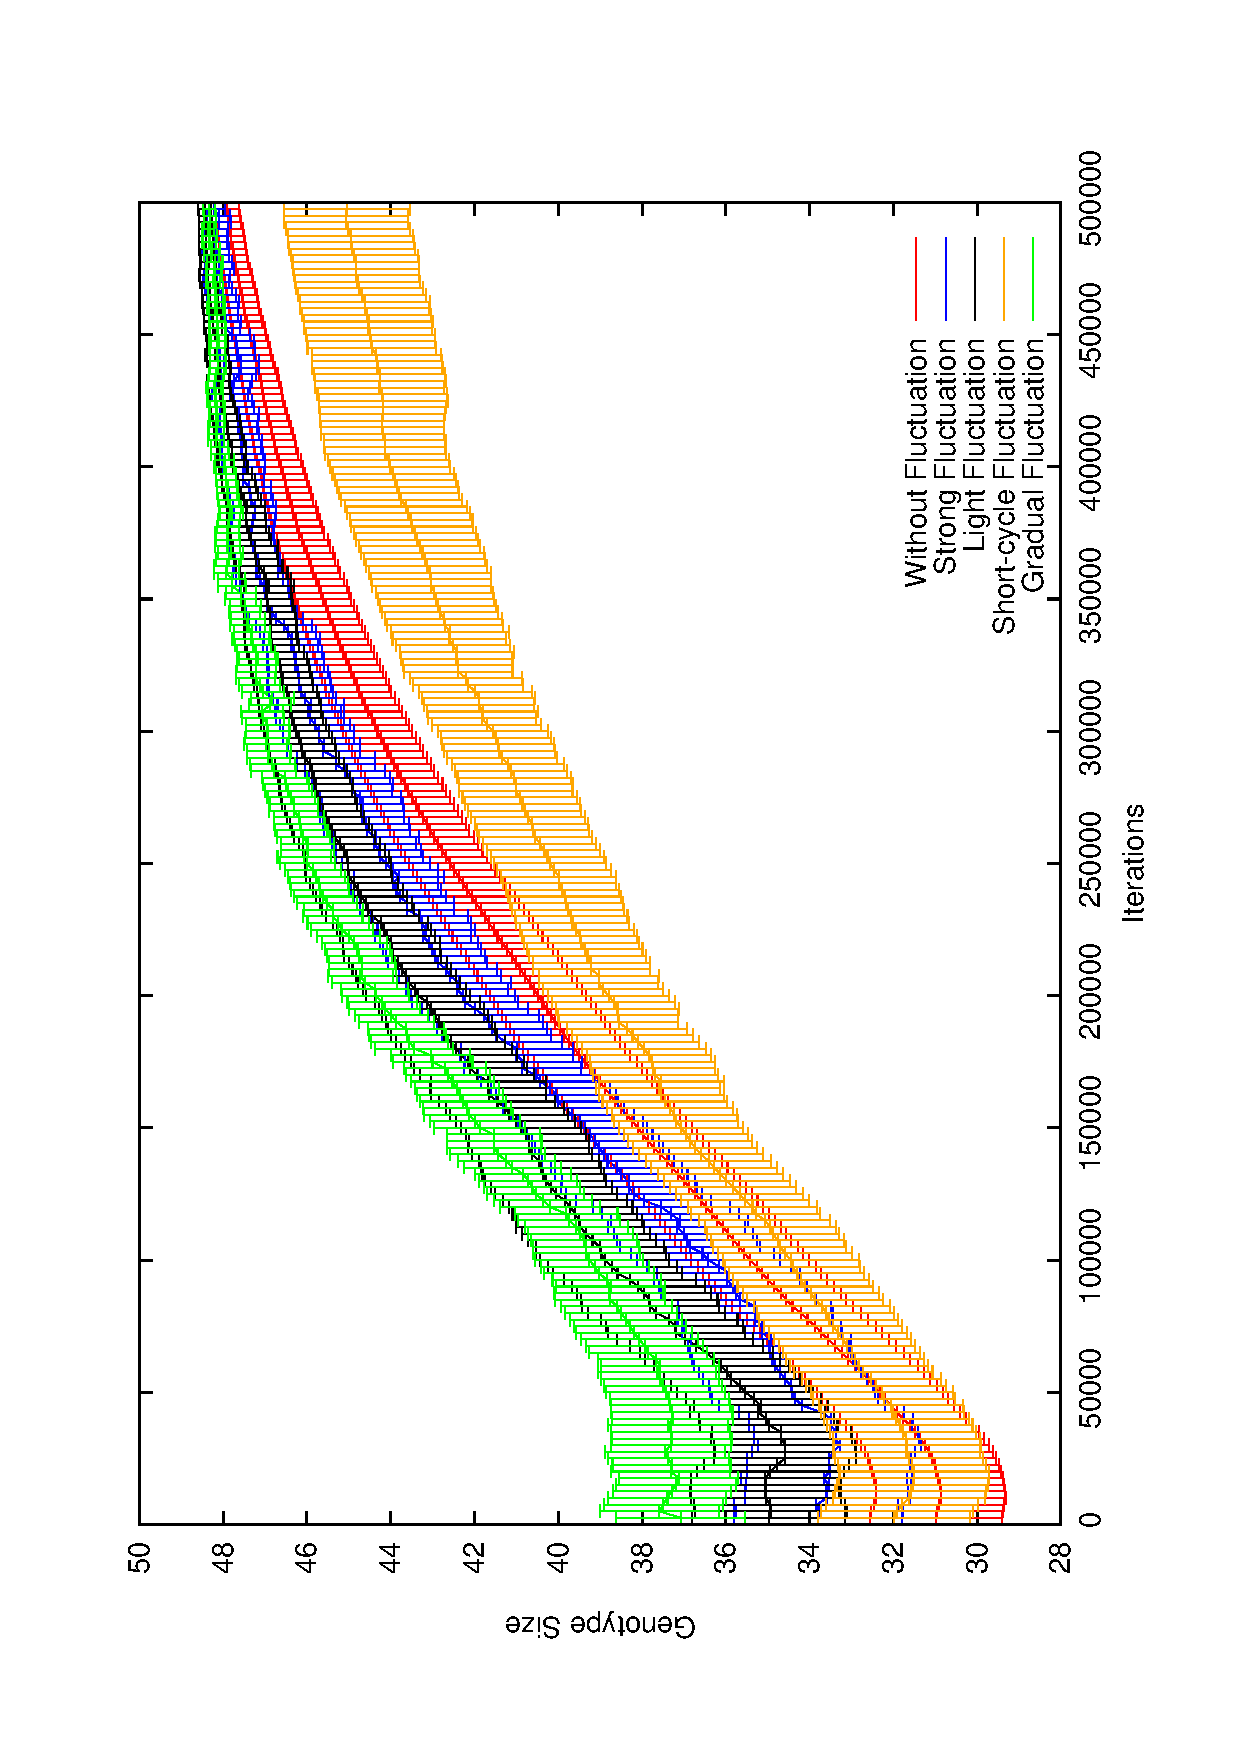
\includegraphics[width=0.7\columnwidth, angle=-90]{img/Size}
\caption{Average genotypes size in number of LGP statements.}
\label{fig:Size}
\end{figure}

\begin{figure}[h]
\centering
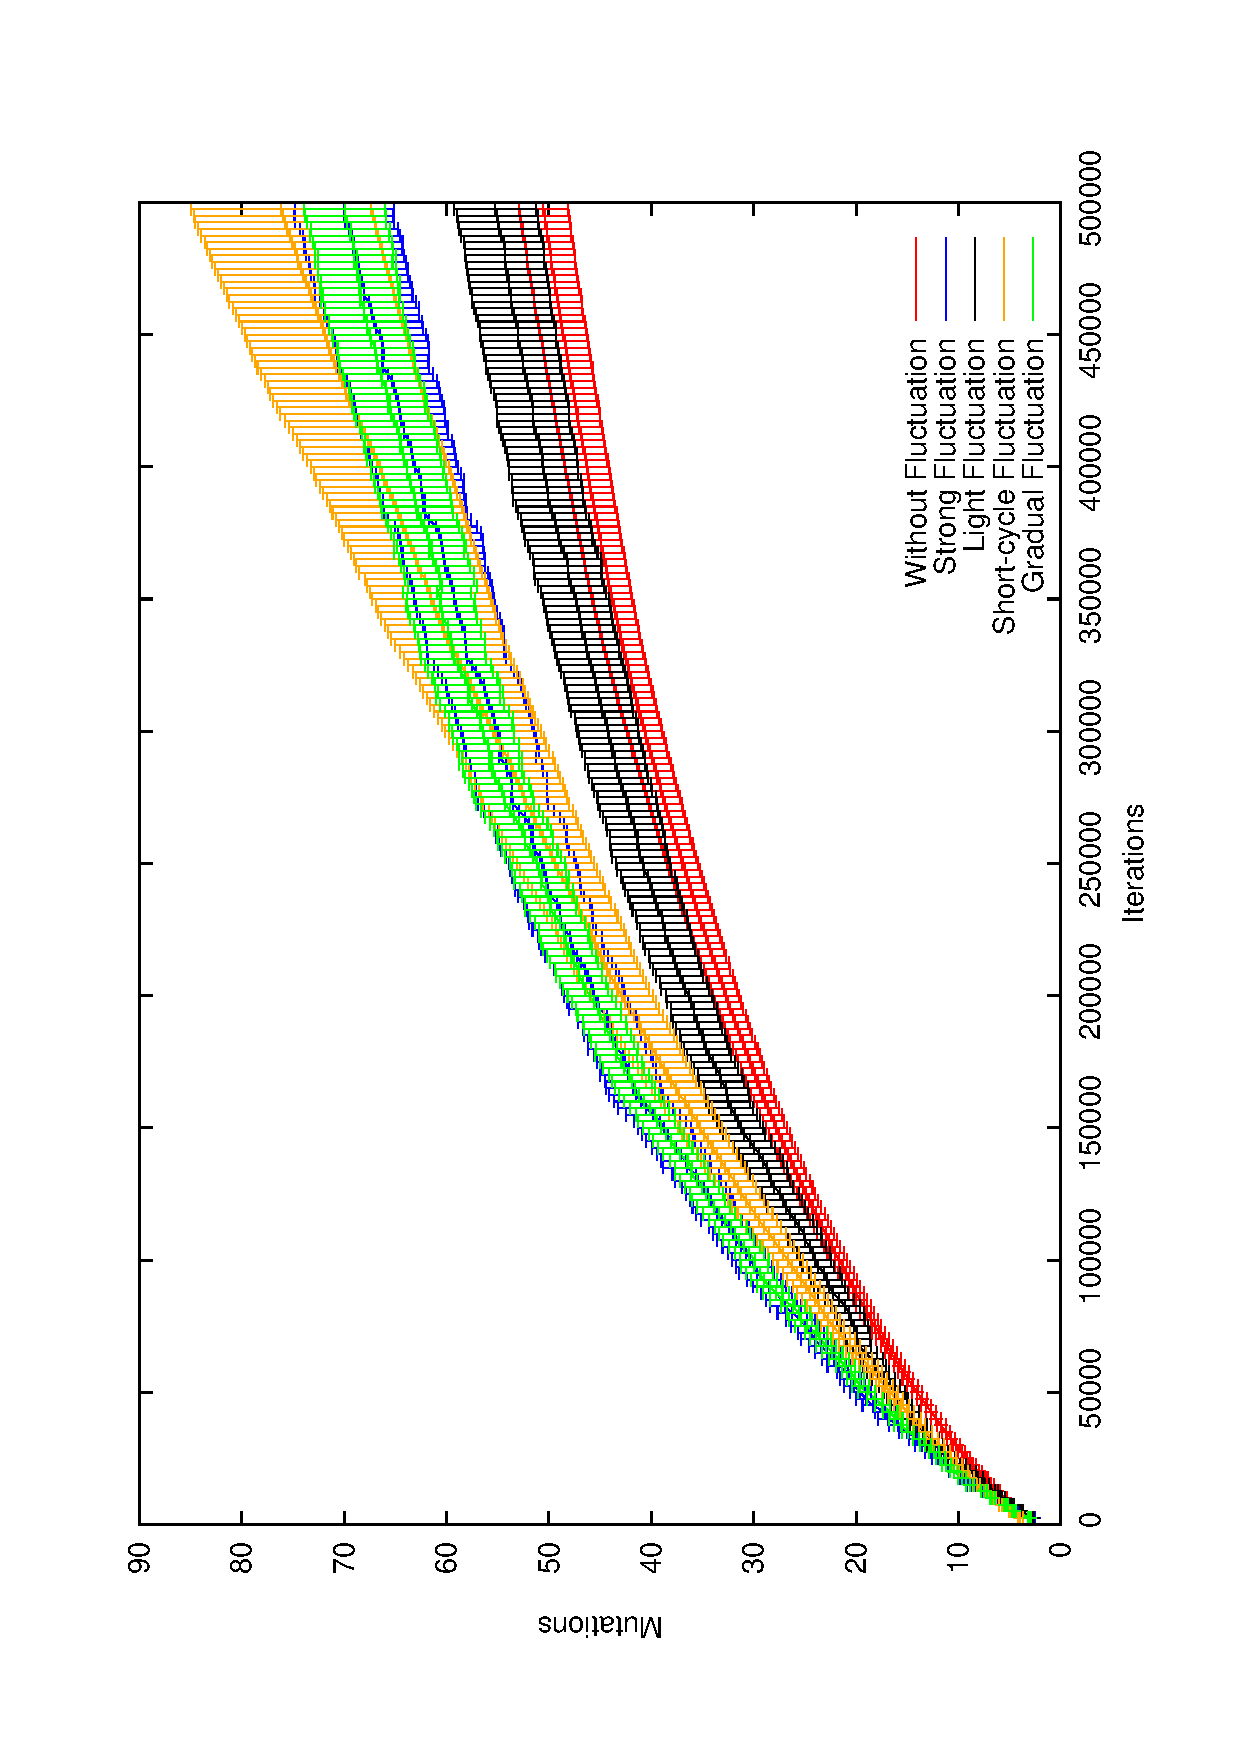
\includegraphics[width=0.7\columnwidth, angle=-90]{img/Mutations}
\caption{Average number of ancestral mutations involved in producing current MCG.}
\label{fig:Mutations}
\end{figure}

\subsection{Phenotypic Comparison}

Figure~\ref{fig:dissimilar} shows the phenotypic comparison $\sigma(t_1, t_2)$ between dissimilar environments, i.e.~at $t_1$ and $t_2 = t_1 - \Delta t$ such that $E(t_1) = E(t_2 + f)$. On can see that the impact of environmental fluctuations decreases quickly for ScF while it remains very high for other types of environmental fluctuations. We also note that the phenotypic difference of ScF remains most of the time lower than the phenotypic differences of the SE. This suggests the selection of a single phenotype, robust in both environments. Figure~\ref{fig:similar} shows $\sigma$ between similar environment, i.e. such that $E(t_1) = E(t_2)$. It can be observed that phenotypic differences in LF and SF are much lower than they are in Figure~\ref{fig:dissimilar}.

\begin{figure}[h]
\centering
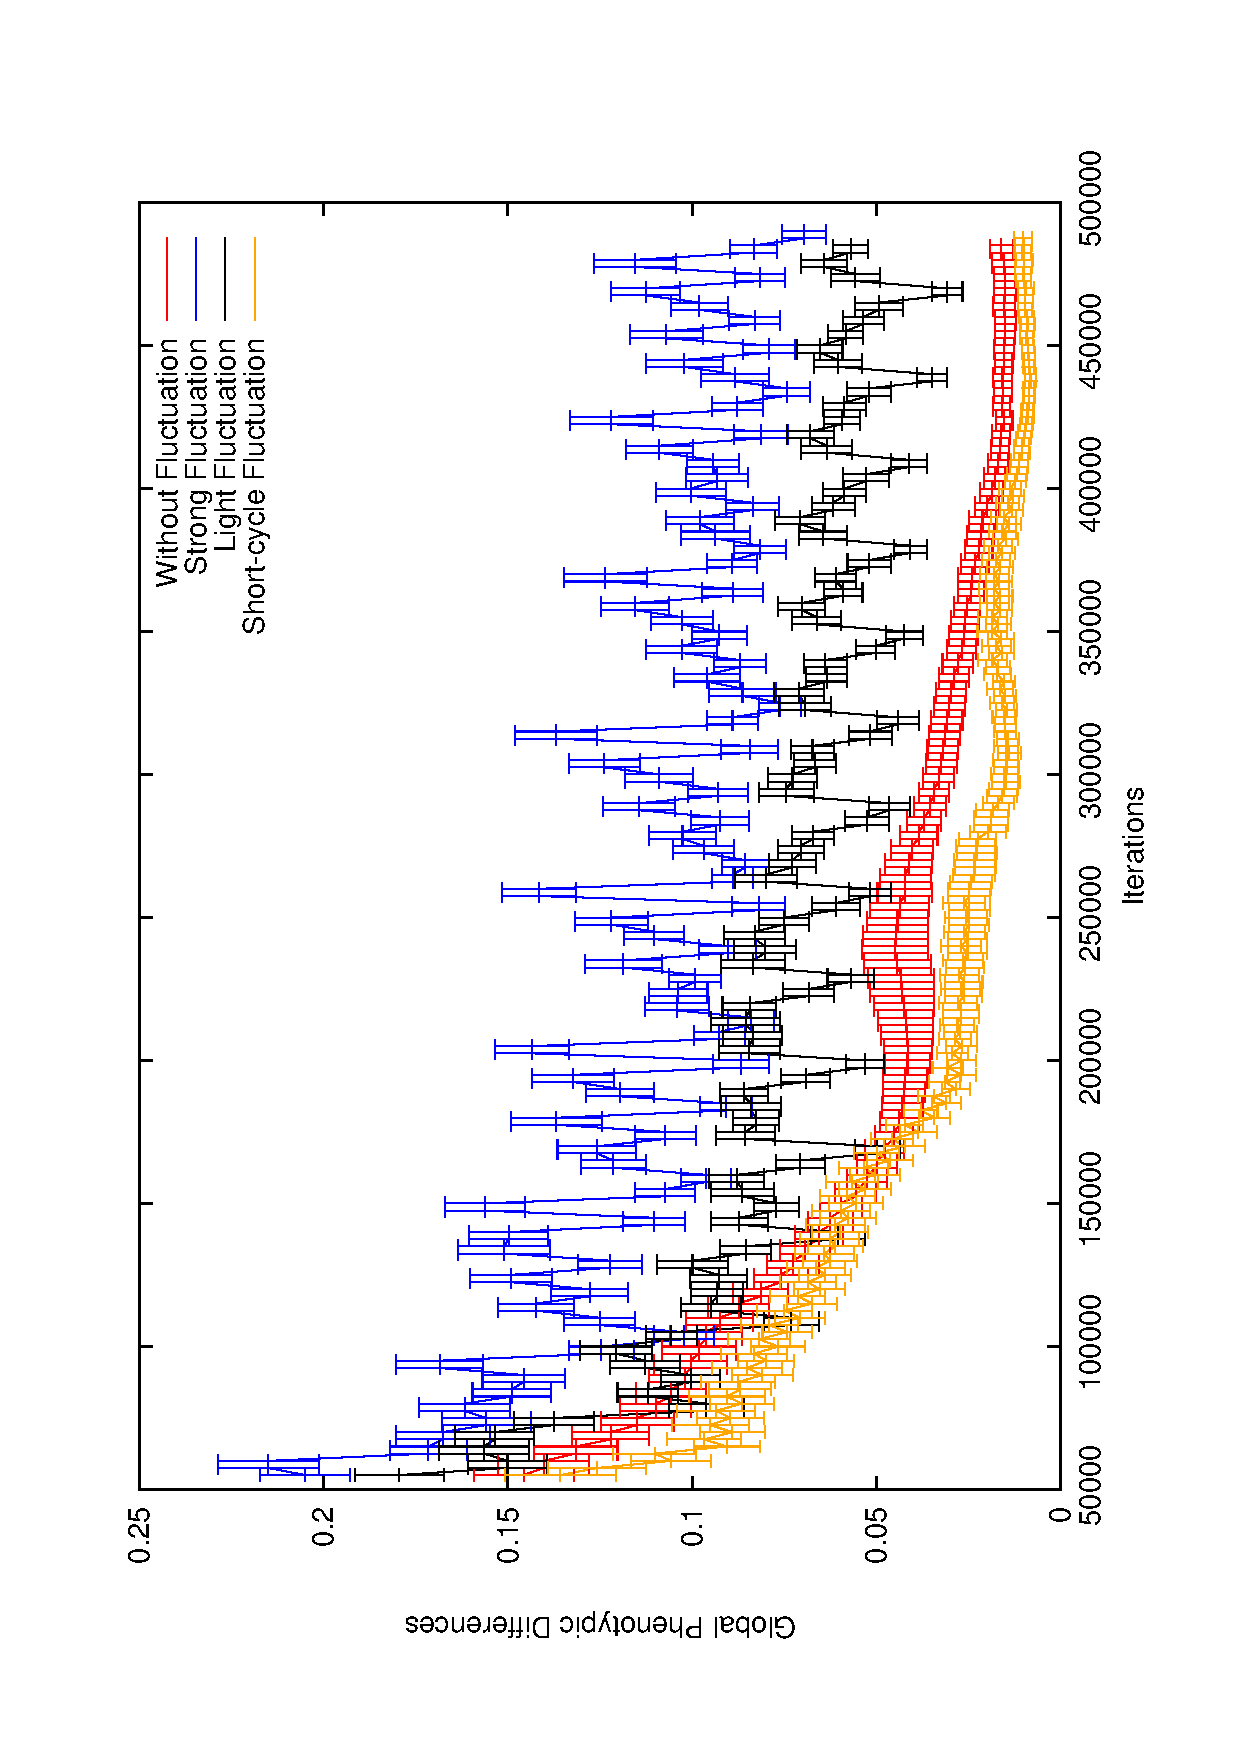
\includegraphics[width=0.7\columnwidth, angle=-90]{img/diffProp}
\caption{Phenotypic comparison $\sigma$: similar environments.}

\label{fig:dissimilar}
\end{figure}
\begin{figure}[h]

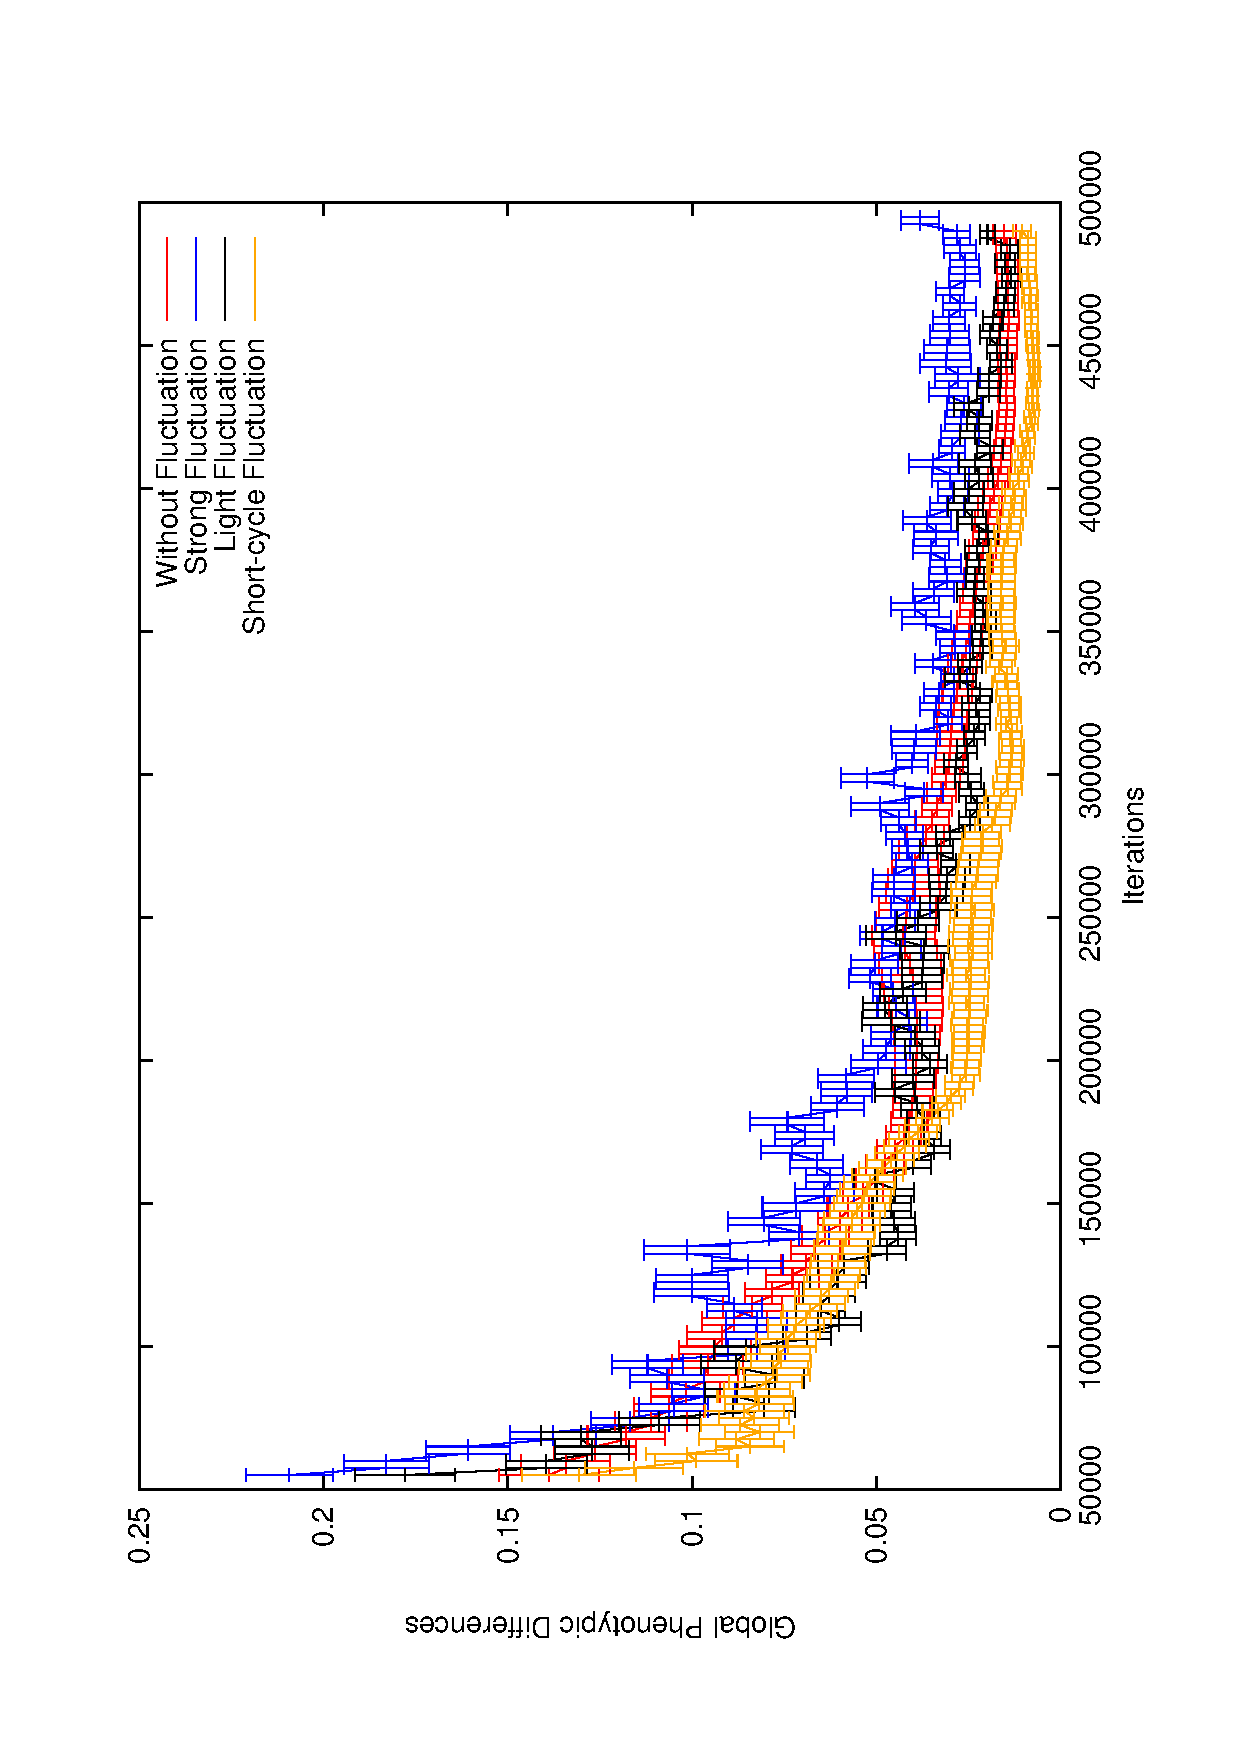
\includegraphics[width=0.7\columnwidth, angle=-90]{img/ProgressProp}
\caption{Phenotypic comparison $\sigma$: dissimilar environments.}
\label{fig:similar}
\end{figure}

\subsection{Phenotypic and Genotypic Diversity}

Figures~\ref{fig:phenodiv} and~\ref{fig:genodiv} depict the average phenotypic and genotypic diversities, $^2\!D_p$ and $^2\!D_g$. The generally low phenotypic diversity of ScF suggests the existence in this configuration of a dominant phenotype, which remains rather stable over time, whereas the relatively high phenotypic diversity of LF and SF combined with a relatively low genotypic diversity might suggest the existence of strong phenotypic selection, hence some form of plasticity.

\begin{figure}[h]
\centering
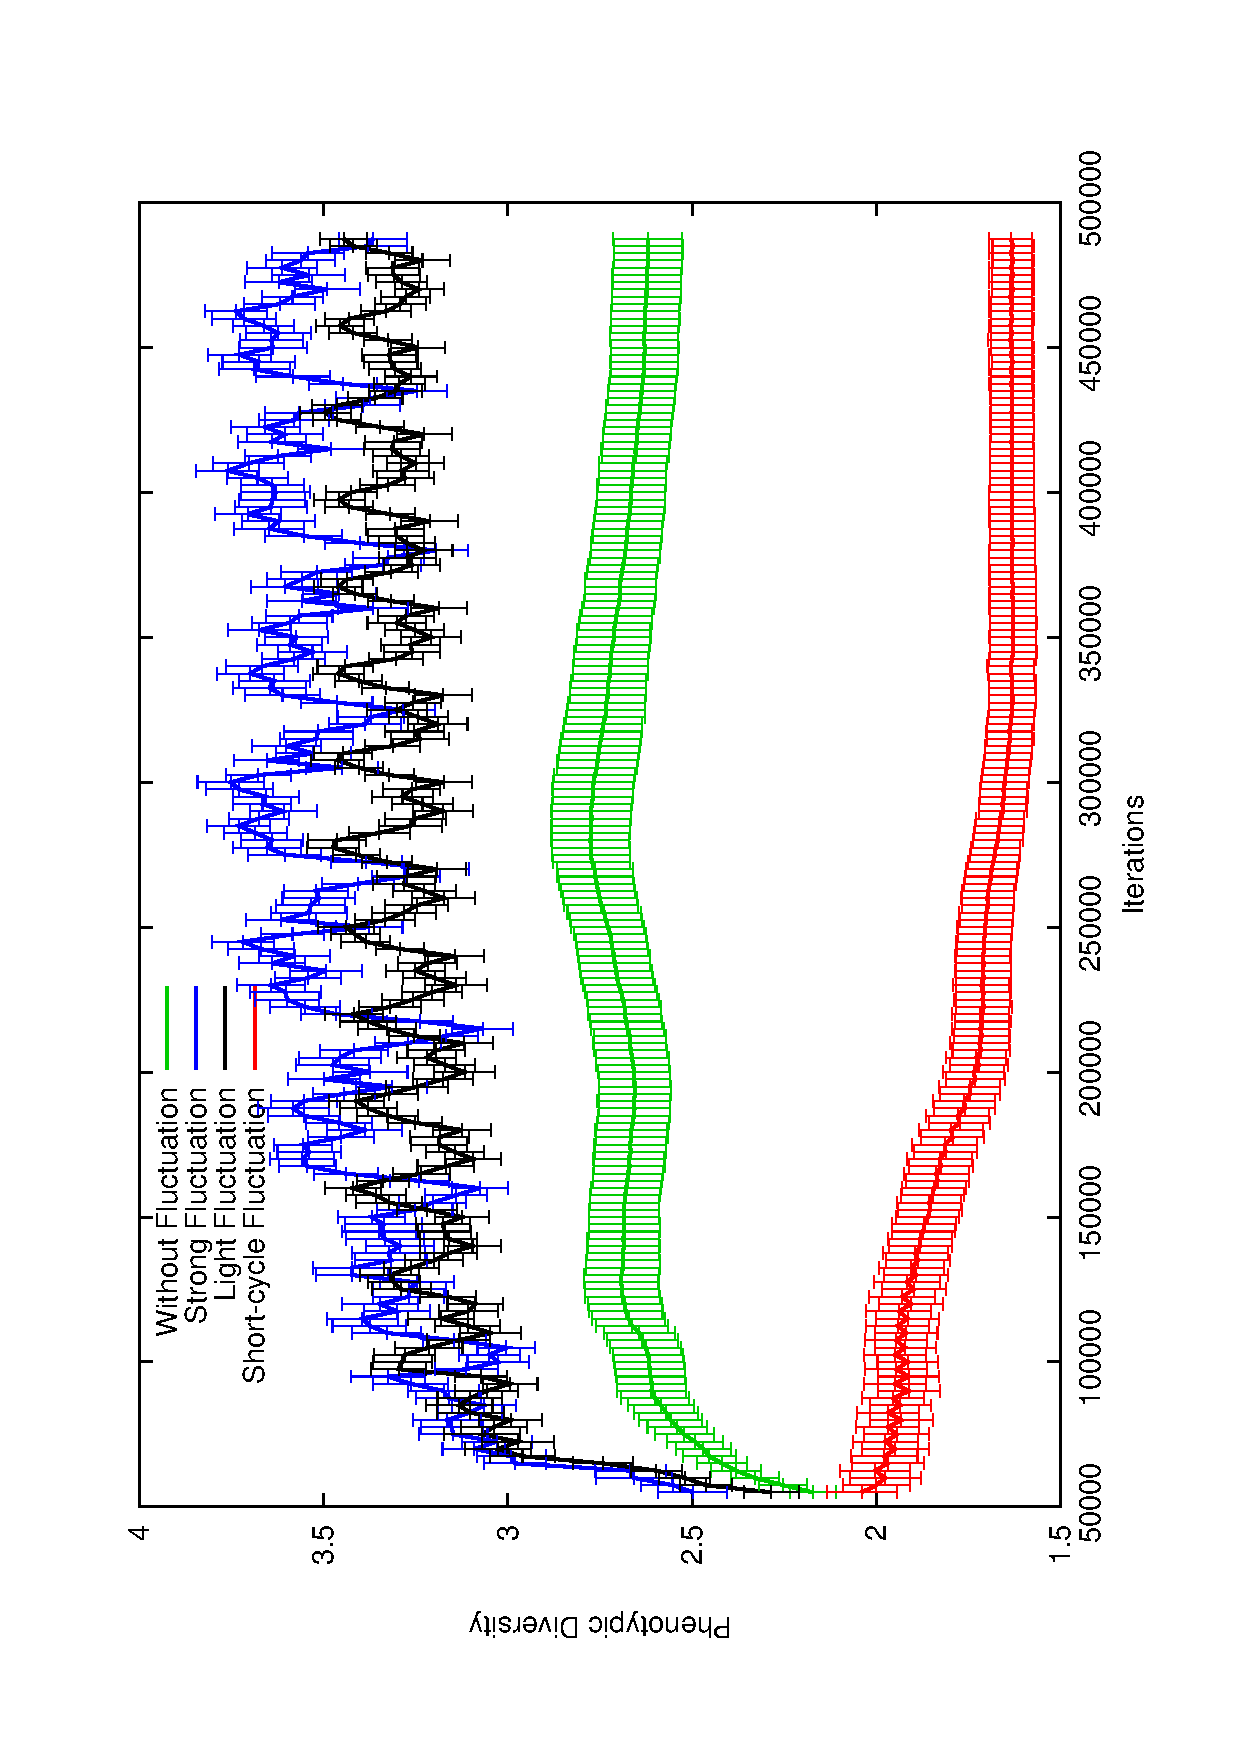
\includegraphics[width=0.7\columnwidth, angle=-90]{img/PhenoDiv}
\caption{Phenotypic diversity.}
\label{fig:phenodiv}
\end{figure}

\subsection{Success Rates of the Homogeneous Test}



Success rates of genotypes in different homogeneous simulations are reported in Figure \ref{fig:survrate} using a normal approximation with a 95\% confidence interval. The fact that SE offers the lowest challenge is not surprising. Similarly the fact that SF is the least conducive to success is also expected. A comparison of the levels of difficulty between LF and ScF is less clear, however, since ScF performs significantly better in its own settings while on the contrary all other tested fluctuations are slightly more efficient in LF. It is also noteworthy that individuals from LF and SF seem relatively robust in various environmental configurations, while those from ScF seem fragile outside the environmental conditions in which they evolved. Moreover, among genotypes collected from iteration 102,500, these same individuals are the only ones that do not reach a 100\% survival ratio in a stable environment.

\subsection{Ending Iteration}

Figure~\ref{fig:ending} displays the last iterations reached by living cells of homogeneous runs of genotypes collected at iteration 100,000 and 500,000. Note that ScF genotypes failures are concentrated around iteration 15,000 in LF homogeneous tests and 25,000 in SF homogeneous tests. This corresponds for these two configurations to the first environment for which $K(S_3) = 0$, whereas $K(S_3) = 1$ for all distributions $E$ in ScF. But we also see that some of the genotypes from ScF fail during the early iterations of the homogeneous test regardless of the environmental fluctuations, including SE and ScF. This might imply that the ecosystem resulting from the evolutionary history of the individuals plays a key role in their ability to survive in ScF.

\begin{figure}[t]
\centering
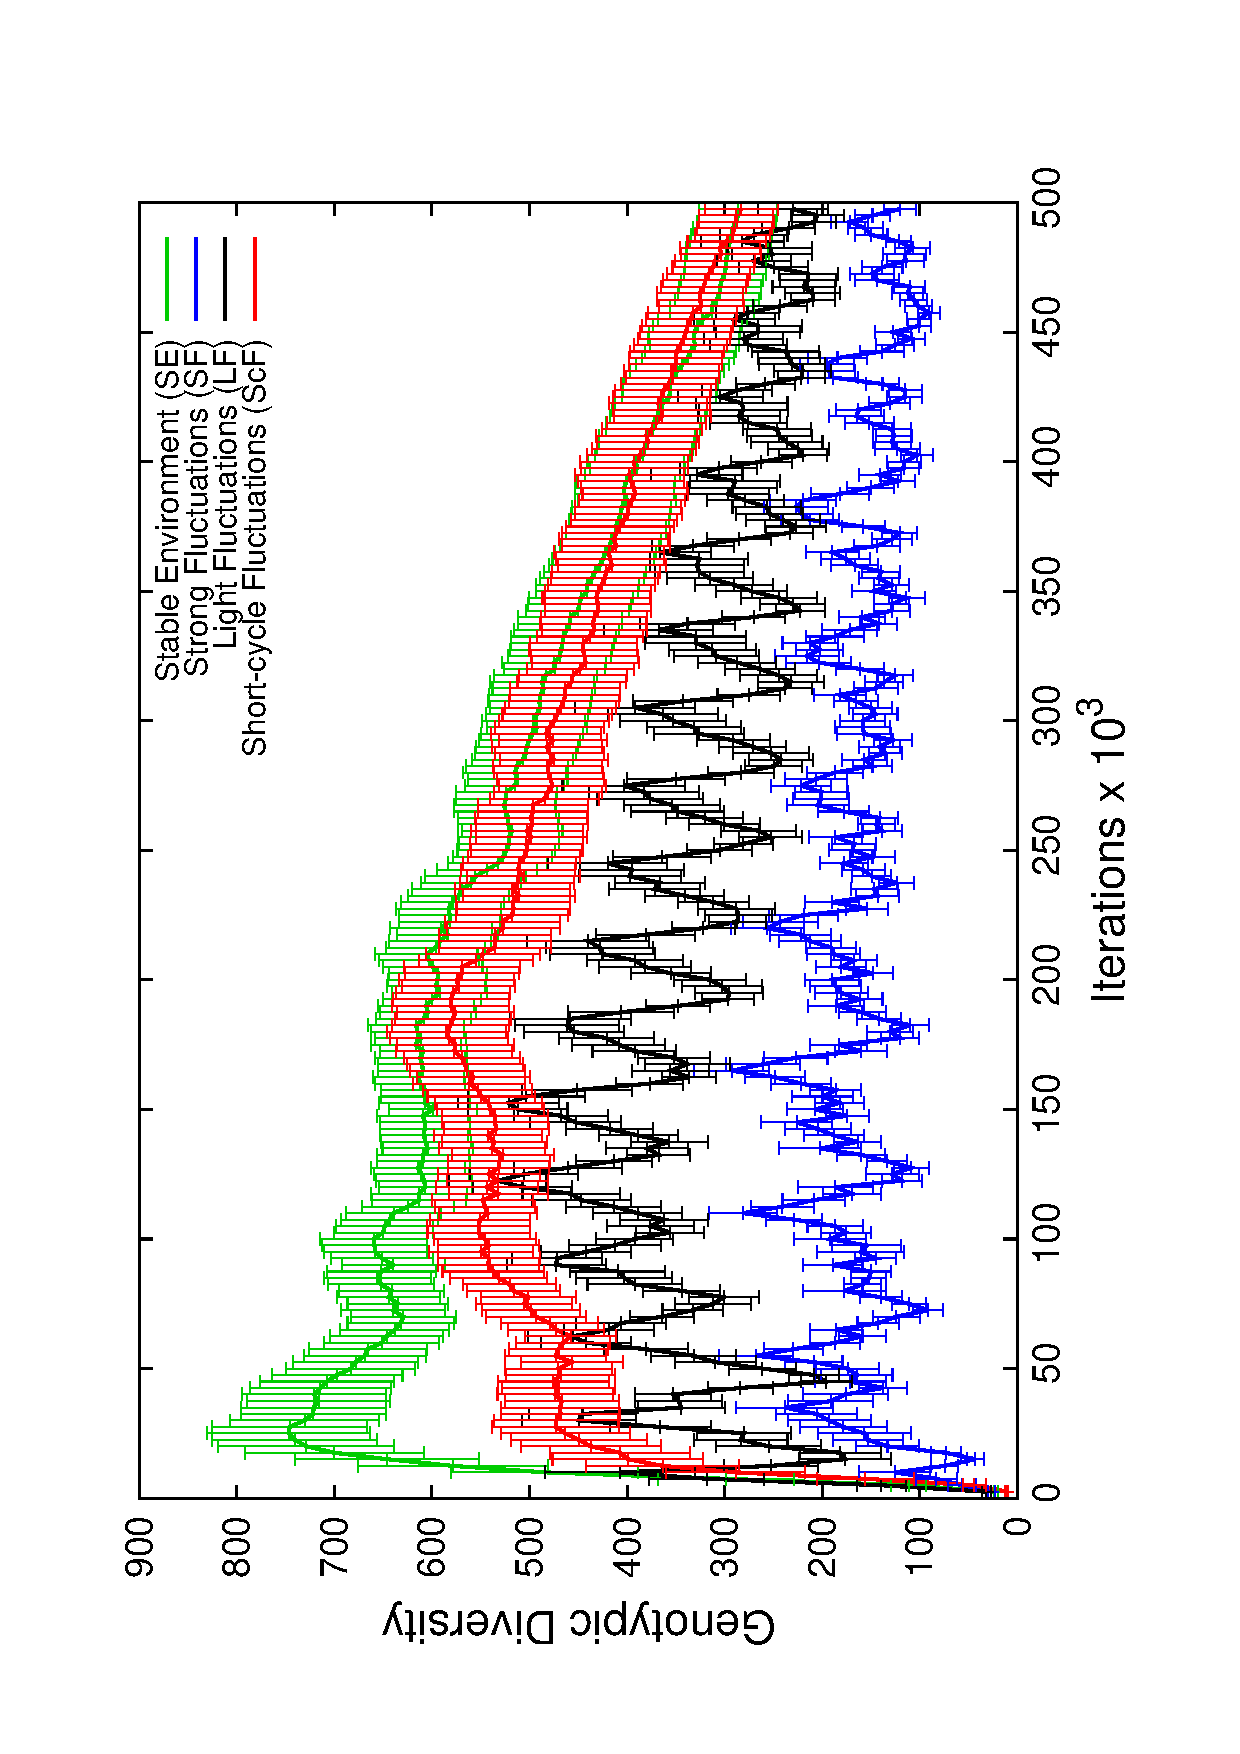
\includegraphics[width=0.7\columnwidth, angle=-90]{img/GenoDiv}
\caption{Genotypic diversity.}
\label{fig:genodiv}
\end{figure}

%\subsection{Phenotypic Densities}
%Figure~\ref{fig:density} depict the density of phenotypes as measured in homogeneous tests. 

%\begin{figure}[H]
%\begin{subfigure}{.25\textwidth}
%  \centering
%  \includegraphics[width=.7\linewidth, angle =-90]{img/boxdensitystable.eps}
%  \caption{Stable environment.}
%  \label{fig:sfig1}
%\end{subfigure}%
%\begin{subfigure}{.25\textwidth}
%  \centering
%  \includegraphics[width=.7\linewidth, angle =-90]{img/boxdensityvariation.eps}
%  \caption{Strong Fluctuation.}
%  \label{fig:sfig2}
%\end{subfigure}

%\begin{subfigure}{.25\textwidth}
%  \centering
%  \includegraphics[width=.7\linewidth, angle =-90]{img/boxdensityvariationLight.eps}
%  \caption{Light Fluctuation.}
%  \label{fig:sfig2}
%\end{subfigure}%
%\begin{subfigure}{.25\textwidth}
%  \centering
%  \includegraphics[width=.7\linewidth, angle =-90]{img/boxdensityvariationSmall.eps}
%  \caption{Small Fluctuation.}
%  \label{fig:sfig1}
%\end{subfigure}
%\caption{Density of Genotype : Each genotype density is processed in four possible different environments.}
%\label{fig:density}
%\end{figure}
